\documentclass[border=5pt]{standalone}
\usepackage{tikz}
\usepackage{amsmath}
\usetikzlibrary{calc,intersections}
\usepackage{pgfplots}
\pgfplotsset{compat=1.16}
\usepgfplotslibrary{polar}
\begin{document}
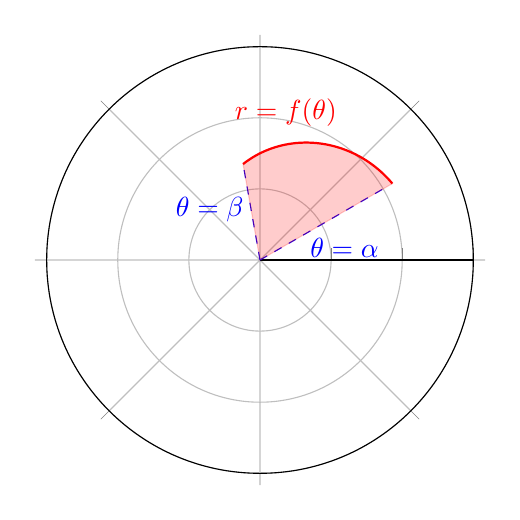
\begin{tikzpicture}
\begin{polaraxis}[
    width=7cm,
    height=7cm,
    grid=both,
    xmin=0, xmax=360,
    ymin=0, ymax=3,
    xtick={0,45,90,135,180,225,270,315},
    ytick={1,2,3},
    xticklabels={},
    xticklabels={},
    yticklabels={},
]
    % Polar curve
    \addplot[red, thick, domain=30:100, samples=100] {1.5*(1+0.5*cos(x))};

    % Bounding rays
    \draw[blue, dashed] (axis cs:30,0) -- (axis cs:30,2);
    \draw[blue, dashed] (axis cs:100,0) -- (axis cs:100,{1.5*(1+0.5*cos(100))});

     % Filled region - properly defined to include the origin
     \pgfplotsset{cycle list={{}}}
     \addplot[red, fill=red, opacity=0.2, domain=30:100, samples=100]
         {1.5*(1+0.5*cos(x)))} -- (axis cs:0,0) -- cycle;


    % Labels
    \node[blue] at (axis cs:8,1.2) {$\theta = \alpha$};
    \node[blue] at (axis cs:135,1) {$\theta = \beta$};
    \node[red] at (axis cs:80,2.1) {$r = f(\theta)$};
\end{polaraxis}
\end{tikzpicture}
\end{document}
